\documentclass[10pt,a4paper]{article} 
\usepackage[utf8]{inputenc}
\usepackage{amsmath}
\usepackage{amsfonts}
\usepackage{amssymb}
\usepackage{graphicx}
\usepackage{epstopdf}
\usepackage[ngerman]{babel}
\usepackage[ngerman]{translator}
\usepackage{listings}
\usepackage[colorlinks=true,
        linkcolor=black,
        citecolor=black,
        filecolor=black,
        pagecolor=black,
        urlcolor=black,
        bookmarks=true,
        bookmarksopen=true,
        bookmarksopenlevel=3,
        plainpages=false,
        pdfpagelabels=true]{hyperref}


%Paket laden
\usepackage[
	nonumberlist, %keine Seitenzahlen anzeigen
	acronym,      %ein Abkürzungsverzeichnis erstellen
	toc,          %Einträge im Inhaltsverzeichnis
	section]      %im Inhaltsverzeichnis auf section-Ebene erscheinen
	{glossaries}
\usepackage{pdfpages}


\parindent 0pt
\pagestyle{headings}

%\let\oldsection\section
%\renewcommand{\section}{\newpage \oldsection}

\title{
	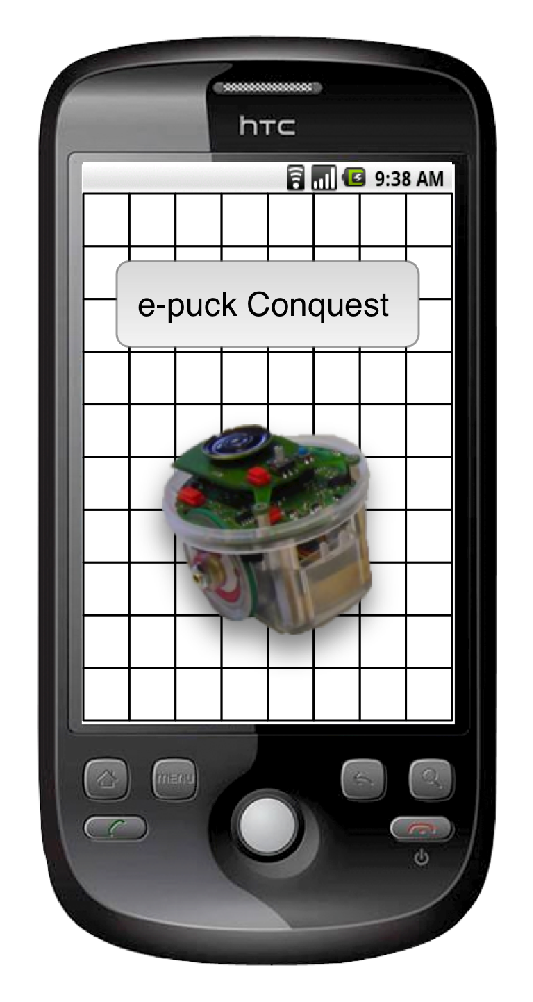
\includegraphics[height=10cm]{logo.eps} \\
%	\vspace{1cm}
	Validierungsbericht
}
\author{
            \begin{tabular}[r]{*{3}{|c|}}
	\hline
	Phase & Verantwortlicher & E-Mail \\
	\hline \hline
	Pflichtenheft & Florian Lorenz & lorenz@fim.uni-passau.de \\
	\hline
	Entwurf & Andreas Wilhelm &  wilhelma@fim.uni-passau.de \\
	\hline
	Spezifikation & Andreas Poxrucker & poxrucke@fim.uni-passau.de \\
	\hline
	Implementierung & Martin Freund & freund@fim.uni-passau.de \\
	\hline
	Validierung & Florian Bürchner & buerchne@fim.uni-passau.de \\
	\hline
	Präsentation & Max Binder & binder@fim.uni-passau.de \\
	\hline
	\end{tabular}
}

\date{21. Januar 2011}
	
	
\begin{document}

	\maketitle
	\newpage
	\tableofcontents
	\newpage

	\begin{abstract}
		Dieses Dokument soll einen Überblick über ...
	\end{abstract}	

	\section{Globale Testszenarien und Testfälle}
		\subsection{Pflichtenheft Testfälle}
			\subsubsection{/T50/ Kalibrierung}
			Nach ordnungsgemäßer Kalibrierung beginnen die Außen-LEDs nacheinander zu leuchten (/F180/).
			
			\subsubsection{/T60/ Linienerkennung}
			Der e-puck wird im Betrieb entlang einer Linie aufgestellt und folgt dieser in Richtung der
			Liniensensoren (/F100/).
			
			\subsubsection{/T70/ Bluetooth-Scan}
			Mehrere e-puck-Roboter werden auf dem Spielfeld platziert und eingeschaltet. Nach der Initialisierungsphase
			sollen sämtliche Teilnehmer auf dem Smartphone erkannt werden (/F200/).
			
			\subsubsection{/T80/ Broadcast-Test}
			Gemäß /T70/ werden alle verbindungsbereiten e-puck Roboter auf dem Suchdialog des Smartphone
			angezeigt. Es wird ein Roboter ausgewählt, alle im Netzwerk befindlichen Teilnehmer werden im Dropdown-Steuerelement
			aufgelistet  (/F50/, /F60/, /F65/, /F70/, /F205/, /F210/).
			
			\subsubsection{/T90/ Knotenanalyse und manuelle Steuerung per On-Screen-Joystick}
			Der Roboter wird gemäß /T60/ aufgestellt. Durch manuelle Steuerung per On-Screen-Joystick muss der
			Benutzer auf allen Knotentypen die möglichen Fahrtrichtungen testen. Nur gültige Richtungen
			dürfen vom Roboter befahren werden (/F80/, /F110/, /F220/, /F270/).
			
			\subsubsection{/T100/ Steuerung der Fahrtgeschwindigkeit}
			Der Roboter wird gemäß \textbf{/T60/} aufgestellt. Bei der manuellen Steuerung per On-Screen-Joystick werden
			sämtliche Geschwindigkeitsstufen überprüft (/F85/).
			
			\subsubsection{/T110/ Steuerung per Beschleunigungssensor}
			Der Test wird analog zu /T80/ durchgeführt, wobei als Steuerungsmethode der Beschleunigungssensor
			verwendet wird (/F280/).
			
			\subsubsection{/T120/ Erkundungstest}
			Mehrere e-puck Roboter werden auf entsprechende Startpositionen innerhalb des Spielfelds gesetzt und
			eingeschaltet. Ziel des Testszenarios ist die vollständige Erkundung durch effiziente Zusammenarbeit der Teilnehmer.
			Falls die Roboter nach Abschluss auf die Startpositionen zurückkehren und die Karte auf dem Smartphone dargestellt
			wird, ist der Testfall erfolgreich (/F90/, /F120/, /F130/, /F135/, /F140/,
			/F150/, /F155/, /F160/, /F190W/, /F230/, /F320/, /F330/).
			
			\subsubsection{/T130/ erweiterter Steuerungstest}
			Der Benutzer wählt nach der Lokalisierung von mindestens zwei Roboter einen per Dropdown-Steuerelement aus.
			Anschließend wird die Steuerung über beide Steuerungsarten (/F270/, /F280/) durchgeführt. Im nächsten
			Schritt wird eine anderer Roboter gewählt und die Steuerung mit diesem geprüft (/F290/, /F300/, /F310/).
			
			\subsubsection{/T140W/ Speichern der Kartendaten}
			Nachdem eine Kartenansicht auf dem Smartphone verfügbar ist, speichert der Benutzer die Kartendaten ab (/F250W/).
			
			\subsubsection{/T150W/ Laden der Kartendaten}
			Nachdem Kartendaten auf dem Smartphone gespeichert wurden (/T120W/), lädt der Benutzer diese.
			Daraufhin wird die entsprechende Karte angezeigt (/F260W/).
			
			\subsubsection{/T160W/ Test von globaler Lokalisierung}
			Die e-puck Roboter werden im Gegensatz zu /T110/ auf beliebigen Startpositionen gesetzt. Somit müssen
			sich die Teilnehmer zunächst finden und synchronisieren. Der erfolgreiche Abschluss kann durch die Anzeige aller e-pucks
			auf der Karte kontrolliert werden (/F170W/).
			
			\subsubsection{/T170W/ Test der Zoomfunktionalität}
			Nach dem Aufbau der Karte auf dem Smartphone werden Fingergesten zum Zoomen sowie Verschieben des
			Kartenausschnittes verwendet. (/F340W/). 

		
		\subsection{weitere Testfälle}
	
	
	\section{Unit Tests}
		\subsection{Android Anwendung}
		
			\subsubsection{GridMap}
			\begin{itemize}
				\item \texttt{testInsertNode()} Ein neuer Knoten wird erstellt und in die GridMap eingefügt. Anschließend wird die GridMap in eine Liste umgewandelt und deren Größe 							abgefragt, um sicherzustellen, dass der Knoten eingefügt wurde.
				\item \texttt{testFrontierNodeRightT()} Ein neuer Knoten wird erstellt und in die GridMap eingefügt. Anschließend wird durch die GridMap eine Liste mit Frontierknoten 							erstellt und überprüft, ob drei Frontierknoten eingefügt wurden.
				\item \texttt{testFrontierNodeLeftT()} Ein neuer Knoten wird erstellt und in die GridMap eingefügt. Anschließend wird durch die GridMap eine Liste mit Frontierknoten 							erstellt und überprüft, ob drei Frontierknoten eingefügt wurden.
				\item \texttt{testFrontierNodeTopT()} Ein neuer Knoten wird erstellt und in die GridMap eingefügt. Anschließend wird durch die GridMap eine Liste mit Frontierknoten 							erstellt und überprüft, ob drei Frontierknoten eingefügt wurden.
				\item \texttt{testFrontierNodeBottomT()} Ein neuer Knoten wird erstellt und in die GridMap eingefügt. Anschließend wird durch die GridMap eine Liste mit Frontierknoten 							erstellt und überprüft, ob drei Frontierknoten eingefügt wurden.
				\item \texttt{testFrontierNodeCross()} Ein neuer Knoten wird erstellt und in die GridMap eingefügt. Anschließend wird durch die GridMap eine Liste mit Frontierknoten 							erstellt und überprüft, ob vier Frontierknoten eingefügt wurden.
				\item \texttt{testFrontierNodeBottomRightEdge()} Ein neuer Knoten wird erstellt und in die GridMap eingefügt. Anschließend wird durch die GridMap eine Liste mit 								Frontierknoten erstellt und überprüft, ob zwei Frontierknoten eingefügt wurden.
				\item \texttt{testFrontierNodeBottomLeftEdge()} Ein neuer Knoten wird erstellt und in die GridMap eingefügt. Anschließend wird durch die GridMap eine Liste mit 								Frontierknoten erstellt und überprüft, ob zwei Frontierknoten eingefügt wurden.
				\item \texttt{testFrontierNodeTopRightEdge()} Ein neuer Knoten wird erstellt und in die GridMap eingefügt. Anschließend wird durch die GridMap eine Liste mit 									Frontierknoten erstellt und überprüft, ob zwei Frontierknoten eingefügt wurden.
				\item \texttt{testFrontierNodeTopLeftEdge()} Ein neuer Knoten wird erstellt und in die GridMap eingefügt. Anschließend wird durch die GridMap eine Liste mit 									Frontierknoten erstellt und überprüft, ob zwei Frontierknoten eingefügt wurden.
				\item \texttt{testUpdateNode()} Es werden zwei neue Knoten erstellt und die GridMap eingefügt. Der zuletzt Eingefügte wird abgerufen und sein Knotentyp überprüft. Außerdem 					wird durch die GridMap erneut eine Liste mit Frontierknoten erstellt und deren Größe, die abhängig von der Wahl der Knotentypen ist, überprüft.
				\item \texttt{testMapBorders()} Es werden vier neue Knoten erstellt und in die GridMap eingefügt. Je nach Wahl der Koordinaten dieser Knoten wird hier die Größe des 							Spielfeldes überprüft. Es werden vier Werte verglichen, der minimale x Wert, der maximale x Wert, der minimale y Wert und der maximale y Wert.
				\item \texttt{testSerialieMapInString()} Ein neuer Knoten wird erstellt und in die GridMap eingefügt. Anschließend wird die serialisiert und in einem String Array 								gespeichert. Dieses Array beinhaltet nun den x, den y Wert und den Knotentyp der zuvor eingefügten Knoten, in genau dieser Reihenfolge. Es wird überprüft, ob sich diese Werte 				entsprechen.
			\end{itemize}
			
			\subsubsection{Behaviour}
			\begin{itemize}
				\item \texttt{testExploreBehaviour()} 
			\end{itemize}
			
			\subsubsection{ComManager}
			\begin{itemize}
				\item \texttt{testAddClientAndSend()}
				\item \texttt{testRemoveClient()}
			\end{itemize}
			
			\subsubsection{AStarPathFinder}
			\begin{itemize}
				\item \texttt{testFindPuckMapNodeMapNodeArray()} 
			\end{itemize}
			
			\subsubsection{Handler}
			\begin{itemize}
				\item \texttt{testSimTurnHandler()} Es wird eine neue Nachricht erzeugt, die aus 32 Byte besteht. Diese enthält einen Nachrichtenschlüssel, der wiederum aus den ersten zwei 					Byte besteht. Nun wird ein VirtualPuckRequest erzeugt, der an den Handler gesendet wird. Der Test ist bestanden, wenn sichn der Handler für seinen Nachrichtentyp zuständig 					fühlt und diese Nachricht bearbeitet.
				\item \texttt{testSimStatusHandler()}
				\item \texttt{testSimSpeedHandler()}
				\item \texttt{testSimResetHandler()}
				\item \texttt{testSimMoveHandler()}
				\item \texttt{testSimLEDHandler()}
				\item \texttt{testPuckStatusHandler()}
				\item \texttt{testPuckRejectHandler()}
				\item \texttt{testPuckOkHandler()}
				\item \texttt{testPuckNodeHitHandler()}
				\item \texttt{testPuckCollisionHandler()}
				\item \texttt{testPuckAbyssHandler()}
				\item \texttt{testFailureRequestHandler()}
				\item \texttt{testDriveRequestHandler()}
				\item \texttt{testControlledRequestHandler()}
				\item \texttt{testCollisionRequestHandler()}
			\end{itemize}
		
		\subsection{E-puck Firmware}
		
			\subsubsection{Ringpuffer}
	
	\section{Blackbox Tests}
	
	\section{kontrollflussorientierte Testverfahren}

				 			
\end{document}
